\documentclass[notes,11pt, aspectratio=169]{beamer}

\usepackage{pgfpages}
% These slides also contain speaker notes. You can print just the slides,
% just the notes, or both, depending on the setting below. Comment out the want
% you want.
\setbeameroption{hide notes} % Only slide
%\setbeameroption{show only notes} % Only notes
%\setbeameroption{show notes on second screen=right} % Both

\usepackage{helvet}
% Lato is used when installed (as on your machine); otherwise Helvetica.
\IfFileExists{lato.sty}{\usepackage[default]{lato}}{}
\usepackage{array}


\usepackage{tikz}
\usepackage{verbatim}
\setbeamertemplate{note page}{\pagecolor{yellow!5}\insertnote}
\usetikzlibrary{positioning}
\usetikzlibrary{snakes}
\usetikzlibrary{calc}
\usetikzlibrary{arrows}
\usetikzlibrary{arrows.meta}
\usetikzlibrary{decorations.markings}
\usetikzlibrary{shapes.misc}
\usetikzlibrary{matrix,shapes,arrows,fit,tikzmark}
\usepackage{amsmath}
\usepackage{amssymb}
\usepackage{mathpazo}
\usepackage{hyperref}
\usepackage{lipsum}
\usepackage{multimedia}
\usepackage{graphicx}
\usepackage{multirow}
\usepackage{dcolumn}
\IfFileExists{bbm.sty}{\usepackage{bbm}}{\providecommand{\mathbbm}{\mathbf}}
\newcolumntype{d}[0]{D{.}{.}{5}}
\usepackage{tabularx}
\newcolumntype{Y}{>{\raggedright\arraybackslash}X}


\usepackage{ragged2e}
\usepackage{parskip}
\usepackage{booktabs}
\usepackage{comment}
\linespread{1}
\setbeamertemplate{footline}[frame number]
\setbeamercolor{questionbox}{bg=blue!10, fg=black}


\setlength{\itemsep}{30pt}
\setlength{\parskip}{10pt}
% Theme
\usetheme{default}



\usepackage{changepage}
\usepackage{appendixnumberbeamer}


\usepackage[space]{grffile}

% These are my colors -- there are many like them, but these ones are mine.
\definecolor{blue}{RGB}{0,114,178}
\definecolor{red}{RGB}{213,94,0}
\definecolor{yellow}{RGB}{240,228,66}
\definecolor{green}{RGB}{0,158,115}

\hypersetup{
  colorlinks=false,
  linkbordercolor = {white},
  linkcolor = {blue}
}


%% I use a beige off white for my background
\definecolor{MyBackground}{RGB}{255,253,218}

%% Uncomment this if you want to change the background color to something else
%\setbeamercolor{background canvas}{bg=MyBackground}

%% Change the bg color to adjust your transition slide background color!
\newenvironment{transitionframe}{
  \setbeamercolor{background canvas}{bg=yellow}
  \begin{frame}}{
    \end{frame}
}

\setbeamercolor{frametitle}{fg=blue}
\setbeamercolor{title}{fg=black}
\setbeamertemplate{footline}[frame number]
\setbeamertemplate{navigation symbols}{}
\setbeamertemplate{itemize items}{-}
\setbeamercolor{itemize item}{fg=blue}
\setbeamercolor{itemize subitem}{fg=blue}
\setbeamercolor{enumerate item}{fg=blue}
\setbeamercolor{enumerate subitem}{fg=blue}
\setbeamercolor{button}{bg=MyBackground,fg=blue,}

\setbeamercolor{section in toc}{fg=blue}
\setbeamercolor{subsection in toc}{fg=red}
\setbeamersize{text margin left=1em,text margin right=1em}

\newenvironment{wideitemize}{\itemize\addtolength{\itemsep}{10pt}}{\enditemize}

% ---------------------------------------------------------------------
% Additions for this talk
% ---------------------------------------------------------------------
\newcommand{\placeholder}[1]{{\color{red}[\textbf{Result to come:} #1]}}
\newcommand{\img}[3]{\IfFileExists{#1}{\includegraphics[width=#2]{#1}}%
  {\fbox{\parbox[c][#3][c]{\dimexpr#2-2\fboxsep-2\fboxrule\relax}{\centering\scriptsize\color{gray}[image: #1]}}}}
\newcommand{\src}[1]{\par\vfill{\scriptsize\color{gray}#1\par}}
\newcommand{\Post}{\mathrm{Post}}

% TikZ styles for the diagrams (defined here, not inside frames)
\tikzset{
  bx/.style={draw=gray!50,fill=gray!8,rounded corners=2pt,align=center,font=\footnotesize,inner sep=3pt},
  bxkey/.style={draw=blue,fill=blue!8,line width=0.8pt,rounded corners=2pt,align=center,font=\footnotesize,inner sep=4pt},
  arr/.style={-{Stealth[length=2.2mm]},line width=0.7pt,color=gray},
  barA/.style={fill=blue,draw=none},
  barN/.style={fill=red,draw=none},
  barI/.style={fill=gray!30,draw=none},
  barOld/.style={draw=gray,dashed,line width=0.5pt},
  diag/.style={every node/.append style={anchor=center},every path/.append style={thin}},
}



\title[]{\textcolor{blue}{Immigrant Owners and Trade Diversification}}
\author[]{Nathanael }
\institute{University of }

\date{ \vspace*{0.5cm} [Seminar, date]\\}


\begin{document}

%%% TIKZ STUFF
\tikzset{
        every picture/.style={remember picture,baseline},
        every node/.style={anchor=base,align=center,outer sep=1.5pt},
        every path/.style={thick},
        }
\newcommand\marktopleft[1]{%
    \tikz[overlay,remember picture]
        \node (marker-#1-a) at (-.3em,.3em) {};%
}
\newcommand\markbottomright[2]{%
    \tikz[overlay,remember picture]
        \node (marker-#1-b) at (0em,0em) {};%
}
\tikzstyle{every picture}+=[remember picture]
\tikzstyle{mybox} =[draw=black, very thick, rectangle, inner sep=10pt, inner ysep=20pt]
\tikzstyle{fancytitle} =[draw=black,fill=red, text=white]
%%%% END TIKZ STUFF

% Title Slide
\begin{frame}
\maketitle
\end{frame}

%=====================================================================
% INTRO
%=====================================================================
\begin{frame}{Canada's trade is highly concentrated in one market}
\begin{columns}[T] % align columns
\begin{column}{.38\textwidth}
\vspace{0.5cm}

  \begin{wideitemize}
    \item Nearly two-thirds of Canadian exporters sell exclusively to the United States.
    \item Most businesses that export goods to non-US destinations also export to the United States.
  \end{wideitemize}
\end{column}%
\hfill%
\begin{column}{.48\textwidth}
  \centering
  \img{Audience Reach Infographic Pie Chart Instagram Post(1).png}{\linewidth}{4.2cm}
\end{column}%
\end{columns}
\src{Source: Statistics Canada, \textit{The Daily}, May 16, 2025.}
\end{frame}


\begin{frame}{
Concentration increases risk%
\only<2->{ and the pressure to diversify}
}
\centering

\vspace{0.3cm}

\begin{columns}[T]
    % LEFT COLUMN -- Vulnerability (always visible)
    \begin{column}{0.48\textwidth}
        \centering
        \img{Screenshot 2026-01-28 risk main.png}{\textwidth}{1.8cm}

        \vspace{0.2cm}

        \img{Screenshot 2026-01-28 113133.png}{\textwidth}{1.8cm}
    \end{column}

    % RIGHT COLUMN -- Diversity (appears on click)
    \begin{column}{0.48\textwidth}
        \centering

        \only<2->{%
            \vspace{0.6cm}

            \img{Screenshot 2026-01-28 div2.png}{\textwidth}{1.8cm}

            \vspace{0.6cm}

            \img{Screenshot 2026-01-28 114741.png}{\textwidth}{1.8cm}
        }
    \end{column}
\end{columns}

\end{frame}


\begin{frame}{But diversification is a firm-level problem, not only a policy choice}
\begin{itemize}
    \item Entering new markets requires information about foreign demand, regulations, and networks.
    \item Costs are lower when language, networks, or institutional familiarity exist (Melitz \& Toubal, 2014)
    \item Search frictions may prevent firms from finding foreign partners (Chaney, 2014; Arkolakis, 2010)
    \item These costs are particularly binding for small/medium firms (Albornoz et al., 2012)
\end{itemize}
\vspace{0.2cm}

\only<2>{\textbf{Immigrant owners may possess origin-country knowledge and networks that reduce these entry costs.}}
\end{frame}


\begin{frame}{Research Questions}
\vspace{0.2cm}

\begin{beamercolorbox}[
    wd=\textwidth,
    sep=10pt,
    center,
    rounded=true,
    shadow=true
]{questionbox}
\textbf{Does immigrant ownership facilitate trade diversification, and through which cost?}
\end{beamercolorbox}

\vspace{0.2cm}

\begin{itemize}\setlength{\itemsep}{6pt}
    \item Do firms enter and/or increase trade with owners' countries of origin?
    \item Through which margin: \textbf{new} country--product relationships, or \textbf{bigger} existing ones?
    \item Do firms adjust their destination mix and trade concentration?
    \item Do effects extend beyond the origin country to surrounding regions?
    \item How quickly do trade patterns adjust?
\end{itemize}

\end{frame}


\begin{frame}{We know immigrant-linked firms trade more with origin countries, but not why}
\begin{itemize}
\item Canadian firms with immigrant owners trade more with owners' origins (Fung, Grekou \& Liu 2019; Fung \& Liu 2025)
\item U.S.\ immigrant-founded firms source from founders' birth countries at lower prices (Chikis \& Saygin 2026)
\end{itemize}
\pause
\vspace{0.1cm}
\begin{columns}[T]
\begin{column}{0.47\textwidth}
\textcolor{blue}{\textbf{Reading 1: owner knowledge}}\\
The owner lowers the cost of trading with $o$.\\
$\Rightarrow$ ownership \emph{changes} trade.
\end{column}
\begin{column}{0.47\textwidth}
\textcolor{blue}{\textbf{Reading 2: sorting}}\\
Immigrants found or buy firms already set up to trade with $o$.\\
$\Rightarrow$ ownership only \emph{labels} those firms.
\end{column}
\end{columns}
\pause
\vspace{0.3cm}
\centering\textbf{Cross-sectional comparisons cannot tell these apart.}
\end{frame}


\begin{frame}{This paper holds the firm fixed and changes the owner}
\vspace{0.2cm}
% Coordinate map (cm):
%  axis (0,0)--(14.0,0); switch tick x=5.8
%  pre  node center (2.8,1.15)  min w=5.4 h=1.2
%  post node center (10.0,1.15) min w=7.4 h=1.2
%  labels below axis: left end, switch, right end
\begin{center}
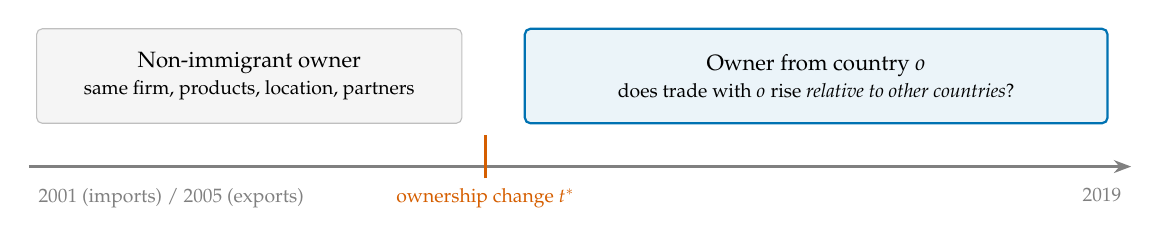
\begin{tikzpicture}[diag]
  \draw[line width=0.8pt,color=gray,-{Stealth[length=2.2mm]}] (0,0) -- (14.0,0);
  \node[bx,minimum width=5.4cm,minimum height=1.2cm] at (2.8,1.15)
     {Non-immigrant owner\\ \scriptsize same firm, products, location, partners};
  \node[bxkey,minimum width=7.4cm,minimum height=1.2cm] at (10.0,1.15)
     {Owner from country $o$\\ \scriptsize does trade with $o$ rise \emph{relative to other countries}?};
  \draw[red,line width=1.4pt] (5.8,-0.15) -- (5.8,0.4);
  \node[font=\scriptsize,color=red,below] at (5.8,-0.15) {ownership change $t^*$};
  \node[font=\scriptsize,color=gray,below right] at (0,-0.15) {2001 (imports) / 2005 (exports)};
  \node[font=\scriptsize,color=gray,below left] at (14.0,-0.15) {2019};
\end{tikzpicture}
\end{center}
\vspace{-0.1cm}
\begin{itemize}\setlength{\itemsep}{4pt}
\item<2-> \textbf{Data}: customs records linked to owners, universe of Canadian traders
\item<3-> \textbf{Variation}: $\approx$1{,}000 incumbent firms switch from non-immigrant to immigrant owners
\item<4-> \textbf{Model}: maps three channels (fixed cost, variable cost, demand) into distinct predictions
\end{itemize}
\note[item]{Convey why there is something to add: new linked data and a new source of variation.}
\end{frame}


\begin{frame}[label=preview]{Preview of findings}
\begin{wideitemize}
\item \placeholder{After an owner from $o$ arrives, trade with $o$ rises by \_\_\% relative to other countries within \_\_ years; no pre-trend.}
\item \placeholder{The increase comes mainly from \_\_ (new country--product pairs / growth of existing flows): the \_\_ channel.}
\item \placeholder{The firm's trade becomes \_\_ concentrated; trade with other partners is \_\_ (created / diverted).}
\end{wideitemize}
\end{frame}


\begin{frame}{Related Literature and Contribution}
\vspace{0.1cm}
\small
\begin{enumerate}\setlength{\itemsep}{4pt}
    \item Immigrant networks and international trade (Gould, 1994; Head \& Ries, 1998; Rauch \& Trindade, 2002; Combes et al., 2005; Parsons \& V\'ezina, 2018)
    \begin{itemize}
      \item \textbf{Contribution}: \textit{within-firm evidence linking ownership transitions to destination-specific trade.}
    \end{itemize}
    \item Immigrant owners, founders and employees in firms' trade (Fung \& Liu, 2025; Cardoso \& Ramanarayanan, 2022; Chikis \& Saygin, 2026)
    \begin{itemize}
      \item \textbf{Contribution}: \textit{tests whether the knowledge moves with the person, holding the business fixed.}
    \end{itemize}
    \item Ownership and strategic firm behaviour (Bloom \& Van Reenen, 2007; Sraer \& Thesmar, 2007)
    \begin{itemize}
      \item \textbf{Contribution}: \textit{ownership identity as a determinant of firms' trade ``capabilities''.}
    \end{itemize}
    \item Margins of trade and trade frictions (Chaney, 2008; Bernard, Redding \& Schott, 2011; Antr\`as, Fort \& Tintelnot, 2017; Morales, Sheu \& Zahler, 2019)
    \begin{itemize}
      \item \textbf{Contribution}: \textit{an observed, person-specific shifter of bilateral fixed and variable costs.}
    \end{itemize}
\end{enumerate}
\end{frame}


\begin{frame}{Roadmap of Talk}
\begin{enumerate}\setlength{\itemsep}{8pt}
\item Data and the ownership switches
\item A model of trade relationships: three channels, three fingerprints
\item Where the model comes from
\item Empirical strategy
\item Results \textcolor{gray}{(to come)}
\end{enumerate}
\end{frame}

%=====================================================================
\begin{transitionframe}
\centering\vfill{\Huge\bfseries Data}\vfill
\end{transitionframe}
%=====================================================================

\begin{frame}{Customs records linked to owners cover every Canadian goods trader}
\vspace{0.2cm}
\renewcommand{\arraystretch}{1.3}
\begin{tabularx}{\textwidth}{@{}p{3.2cm}Yp{3.2cm}@{}}
\toprule
\textbf{Source} & \textbf{What it gives us} & \textbf{Years}\\
\midrule
TIC (imports) & firm $\times$ HS6 product $\times$ source country & 2001--2019\\
TEC (exports) & firm $\times$ HS8 product $\times$ destination (to HS6) & 2005--2019\\
CEEDD & firms, owners, employment & 2001--2019\\
IMDB & owner is an immigrant; country of origin & landing records\\
\bottomrule
\end{tabularx}
\vspace{0.3cm}

\textbf{New here}: owner origin linked to the full product-by-country trade portfolio, \emph{followed through a change of owner}.
\src{Merchandise trade only; trade values (no quantities). Main window 2005--2019 for both directions.}
\end{frame}


\begin{frame}{About 1,000 incumbent firms switch to immigrant owners}
\begin{columns}[T]
\begin{column}{0.5\textwidth}
\textbf{Event}: first year $t^*$ a firm passes to immigrant ownership; $o$ = origin of the new owner

\textbf{Not} conditioned on surviving or trading afterward

\textbf{Excluded}: mergers, consolidations, identifier changes
\end{column}
\begin{column}{0.46\textwidth}
\textbf{Comparison firms}
\begin{itemize}\setlength{\itemsep}{4pt}
\item never sold
\item sold to another non-immigrant\\ {\scriptsize\color{gray}same disruption of a sale}
\item sold to an immigrant from another origin\\ {\scriptsize\color{gray}same selection into immigrant ownership}
\end{itemize}
\end{column}
\end{columns}
\vspace{0.2cm}
\placeholder{Figure: number of switches by year and by origin region.}
\end{frame}

%=====================================================================
\begin{transitionframe}
\centering\vfill{\Huge\bfseries Model}\vfill
\end{transitionframe}
%=====================================================================

\begin{frame}{The model in words: each trade relationship has to clear a bar}
A firm already runs its business. For each \textbf{country} and \textbf{product}, it decides whether a trade relationship is worth having, and how much to trade through it.
\pause
\begin{columns}[T]
\begin{column}{0.31\textwidth}
\textcolor{blue}{\textbf{Fixed costs}}\\ {\small finding a partner, learning the rules, a first contract. Paid to \emph{have} a relationship.}
\end{column}
\begin{column}{0.31\textwidth}
\textcolor{blue}{\textbf{Variable cost}}\\ {\small contracting, monitoring, enforcement, shipping. Paid on every unit \emph{traded}.}
\end{column}
\begin{column}{0.31\textwidth}
\textcolor{red}{\textbf{The owner from $o$}}\\ {\small knows part of what others must learn, \emph{for country $o$ only}.}
\end{column}
\end{columns}
\pause
\vspace{0.3cm}
\centering\textbf{Which cost the owner lowers determines \emph{how} trade with $o$ changes.}
\end{frame}


\begin{frame}{Fixed-cost cuts add relationships; variable-cost cuts grow them}
% Coordinate map (cm). Panel A origin (0,0); Panel B origin (7.6,0).
%  bars: width 0.6, x-left = 0.4 + 0.95*k (k=0..5)
%  A heights 2.4,1.9,1.5,1.1,0.75,0.45 ; old cut y=1.3 ; new cut y=0.9
%  B old heights same (dashed) ; new heights x1.3 = 3.12,2.47,1.95,1.43,0.98,0.59 ; cut y=1.3
%  cut labels at x=6.05 (A) and x=13.65 (B), anchor west
%  panel titles at y=3.55 ; Panel B appears on the second click
\begin{center}
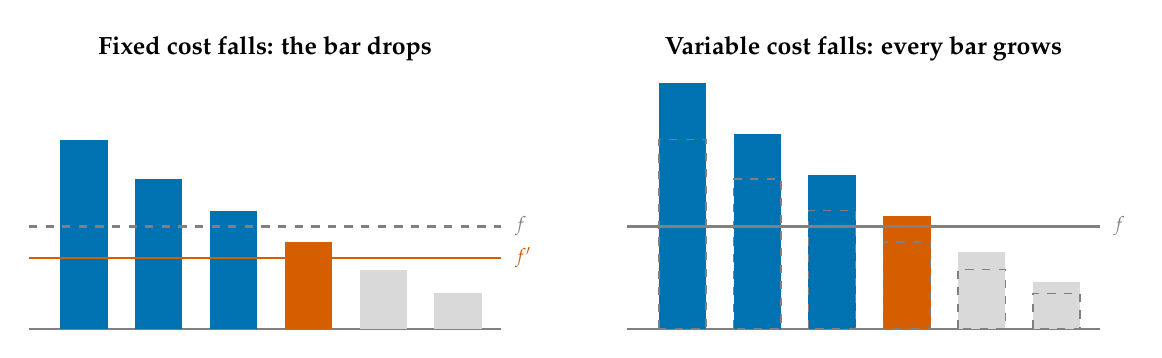
\begin{tikzpicture}[diag]
  % ---- Panel A
  \node[font=\small\bfseries] at (3.0,3.55) {Fixed cost falls: the bar drops};
  \draw[color=gray,line width=0.6pt] (0,0) -- (6.0,0);
  \fill[barA] (0.40,0) rectangle (1.00,2.40);
  \fill[barA] (1.35,0) rectangle (1.95,1.90);
  \fill[barA] (2.30,0) rectangle (2.90,1.50);
  \fill[barN] (3.25,0) rectangle (3.85,1.10);
  \fill[barI] (4.20,0) rectangle (4.80,0.75);
  \fill[barI] (5.15,0) rectangle (5.75,0.45);
  \draw[color=gray,dashed,line width=0.9pt] (0,1.3) -- (6.0,1.3);
  \draw[color=red,line width=0.9pt] (0,0.9) -- (6.0,0.9);
  \node[font=\scriptsize,color=gray,anchor=west] at (6.05,1.3) {$f$};
  \node[font=\scriptsize,color=red,anchor=west] at (6.05,0.9) {$f'$};
  % ---- Panel B (second click)
  \onslide<2->{
  \node[font=\small\bfseries] at (10.6,3.55) {Variable cost falls: every bar grows};
  \draw[color=gray,line width=0.6pt] (7.6,0) -- (13.6,0);
  \fill[barA] (8.00,0) rectangle (8.60,3.12);
  \fill[barA] (8.95,0) rectangle (9.55,2.47);
  \fill[barA] (9.90,0) rectangle (10.50,1.95);
  \fill[barN] (10.85,0) rectangle (11.45,1.43);
  \fill[barI] (11.80,0) rectangle (12.40,0.98);
  \fill[barI] (12.75,0) rectangle (13.35,0.59);
  \draw[barOld] (8.00,0) rectangle (8.60,2.40);
  \draw[barOld] (8.95,0) rectangle (9.55,1.90);
  \draw[barOld] (9.90,0) rectangle (10.50,1.50);
  \draw[barOld] (10.85,0) rectangle (11.45,1.10);
  \draw[barOld] (11.80,0) rectangle (12.40,0.75);
  \draw[barOld] (12.75,0) rectangle (13.35,0.45);
  \draw[color=gray,line width=0.9pt] (7.6,1.3) -- (13.6,1.3);
  \node[font=\scriptsize,color=gray,anchor=west] at (13.65,1.3) {$f$};
  }
\end{tikzpicture}
\end{center}
{\footnotesize Bar = one product the firm could trade with $o$; height = its variable profit.
\textcolor{blue}{$\blacksquare$}~active \quad \textcolor{red}{$\blacksquare$}~newly active \quad \textcolor{gray!50}{$\blacksquare$}~not worth it \quad dashed = before}
\note[item]{Left: only new relationships appear; existing ones are unchanged. Right: existing ones all grow by the same proportion, and a marginal one crosses the bar.}
\end{frame}


\begin{frame}{Setup: a relationship pays variable profit minus fixed costs at two levels}
\begin{columns}[T]
\begin{column}{0.55\textwidth}
Relationship $(c,k,d)$: country $c$, product $k$, direction $d$
\[
\pi_{ickd} \;=\; \underbrace{\Phi_{ickd}\,\tau_{icd}^{-\varepsilon_d}}_{\text{variable profit}} \;-\; \underbrace{f_{ickd}}_{\text{product fixed cost}}
\]
plus a \textbf{country} fixed cost $F_{icd}$ if anything is traded with $c$:
\[
\Pi_i=\sum_{d}\sum_{c\in\mathcal C_{id}}\Big[\sum_{k\in\mathcal K_{icd}}\pi_{ickd}-F_{icd}\Big]
\]
\end{column}
\begin{column}{0.4\textwidth}
\small
$\Phi$: firm scale, demand or supply in $c$, prices\\
$\tau$: variable cost of trading with $c$\\
$\varepsilon$: how much profit reacts to $\tau$\\
Trade value $X_{ickd}\propto\Phi\,\tau^{-\varepsilon}$

\pause
\textbf{Rule}: trade product $k$ if $\Phi\tau^{-\varepsilon}\ge f$; trade with $c$ at all if the sum of those surpluses $\ge F$.
\end{column}
\end{columns}
\note[item]{The Bernard-Redding-Schott two-tier fixed-cost structure at the level of one firm, with firm-specific costs. Separable baseline; the same reduced form covers exporters, importers for resale and input importers (CES).}
\end{frame}


\begin{frame}{The owner removes part of the \emph{information} cost, only for country $o$}
\begin{align*}
\ln\tau_{icd} &= \ln\bar\tau_{cd} + (1-\textcolor{red}{\lambda_\tau D_{ic}})\,\iota_c && \text{variable cost}\\
F_{icd} &= \bar F_{cd} + (1-\textcolor{red}{\lambda_F D_{ic}})\,\psi_c && \text{country fixed cost}\\
f_{ickd} &= \bar f_{ckd} + (1-\textcolor{red}{\lambda_f D_{ic}})\,\psi_{ck} && \text{product fixed cost}
\end{align*}
\begin{itemize}\setlength{\itemsep}{4pt}
\item $D_{ic}=1$ if $c$ is the owner's origin; $\bar\tau,\bar F,\bar f$ are faced by every Canadian firm
\item $\iota,\psi$: the \emph{information} part. The owner removes a share $\lambda$ of it
\item<2-> \textbf{Key assumption}: $\iota,\psi$ are larger where public information is scarce (differentiated goods, weak institutions, distant languages, thin Canada--$c$ trade)
\end{itemize}
\note[item]{If the owner cut tau by a constant proportion everywhere, there would be no heterogeneity to test.}
\end{frame}


\begin{frame}{The competing story: the owner shifts demand, not costs}
\[
\Phi_{ick,\mathrm{im}}=\bar\Phi_{ick,\mathrm{im}}\big(1+\textcolor{red}{\eta}\,D_{ic}\,\mathbbm{1}[k\ \text{consumer good}]\big)
\]
\begin{itemize}
\item e.g.\ an owner serving co-ethnic customers imports more home-country consumer goods
\item<2-> \textbf{Testable}: demand for home goods should \emph{not} raise exports to $o$, or imports of intermediate inputs from $o$
\item<3-> \textcolor{gray}{Weak point: co-ethnic demand for inputs, or trust in home suppliers, would look like a cost channel}
\end{itemize}
\end{frame}


\begin{frame}[label=fingerprints]{Each channel leaves a different fingerprint in the data}
\footnotesize
\renewcommand{\arraystretch}{1.3}
\begin{tabularx}{\textwidth}{@{}>{\raggedright\arraybackslash}p{3.3cm}YYYY@{}}
\toprule
 & \textbf{Country fixed cost} & \textbf{Product fixed cost} & \textbf{Variable cost} & \textbf{Demand}\\
\midrule
Trade with $o$ vs.\ others & rises & rises & rises & consumer imports only\\
Existing $(o,k)$ flows & \textcolor{red}{unchanged} & \textcolor{red}{unchanged} & \textcolor{blue}{all grow by $\varepsilon\lambda_\tau\iota_o$} & consumer imports grow\\
New $(o,k)$ pairs & firms new to $o$, in bundles & one at a time & only near the bar & consumer goods\\
Exports \& input imports & rise & rise & rise & \textcolor{red}{no change}\\
Timing & gradual (search) & gradual (search) & immediate & immediate\\
\bottomrule
\end{tabularx}
\vspace{0.2cm}

\normalsize
\textbf{Margins} separate fixed from variable costs; \textbf{direction and goods type} separate costs from demand.
\end{frame}


\begin{frame}{Interacting sources do not break the within-firm comparison}
\begin{columns}[T]
\begin{column}{0.5\textwidth}
A cheaper source lowers the firm's costs and raises its scale, changing what it buys \emph{everywhere} (Antr\`as, Fort \& Tintelnot 2017, eq.\ 12):
\[
M_{ij}\;\propto\;T_j(\tau_{ij}w_j)^{-\theta}\;\Theta_i^{(\sigma-1-\theta)/\theta}
\]
\end{column}
\begin{column}{0.46\textwidth}
\textbf{An owner who lowers $\tau_{io}$:}
\begin{itemize}\setlength{\itemsep}{4pt}
\item all other countries move by the \textbf{same proportion}: up if $(\sigma-1)/\theta>1$, down if $<1$
\item $o$ relative to any other country moves by exactly $\theta\lambda_\tau\iota_o$
\end{itemize}
\end{column}
\end{columns}
\pause
\vspace{0.2cm}
Firm-by-year effects absorb the common part. \textbf{Creation vs.\ diversion} needs a comparison \emph{across} firms.
\note[item]{Our separable baseline is AFT's knife-edge case (sigma-1)/theta = 1.}
\end{frame}


\begin{frame}{More trade with $o$ diversifies the firm only if $o$ starts out small}
\begin{columns}[T]
\begin{column}{0.47\textwidth}
Herfindahl across partners, $H_i=\sum_c s_{ic}^2$:
\[
\frac{\partial H_i}{\partial X_{io}}=\frac{2}{X_i}\big(\textcolor{red}{s_{io}}-H_i\big)
\]
\end{column}
\begin{column}{0.47\textwidth}
\begin{itemize}\setlength{\itemsep}{4pt}
\item Concentration falls when $o$'s share is below $H_i$
\item For a U.S.-dominated firm, $H_i\approx$ U.S.\ share, so almost any non-U.S.\ origin diversifies it
\end{itemize}
\end{column}
\end{columns}
\pause
\vspace{0.3cm}
Firm-level and national diversification line up when the new trade is \emph{created}, not diverted from non-U.S.\ partners.
\end{frame}


\begin{frame}{Buyers may select on levels of opportunity, not on coming shocks}
A buyer from $o$ values firm $i$ at $V_i+G_i(o)$; the gain $G_i(o)$ is larger for firms whose products $o$ supplies or buys.
\pause
\begin{columns}[T]
\begin{column}{0.47\textwidth}
\textcolor{green}{\textbf{Fine for the design}}\\
{\small Selection on the \emph{level} of fit with $o$: absorbed by firm $\times$ country $\times$ product effects. The estimand is the effect on acquired firms (ATT).}
\end{column}
\begin{column}{0.47\textwidth}
\textcolor{red}{\textbf{Breaks the design}}\\
{\small Selection on a coming \emph{change}, e.g.\ a buyer who knows a contract with $o$ is in prospect.}
\end{column}
\end{columns}
\note[item]{The identifying assumption stated in economic terms.}
\end{frame}

%=====================================================================
\begin{transitionframe}
\centering\vfill{\Huge\bfseries Where the model comes from}\vfill
\end{transitionframe}
%=====================================================================

\begin{frame}{The model is assembled from standard, well-tested parts}
% Coordinate map (cm):
%  left nodes center x=2.9, text width 5.4, min h=0.8; y = 4.32, 3.24, 2.16, 1.08, 0.0
%  right node center (10.6,2.16) text width 4.8, min h=2.6
%  arrows: left.east -> right.west ; note at (2.9,5.0)
\begin{center}
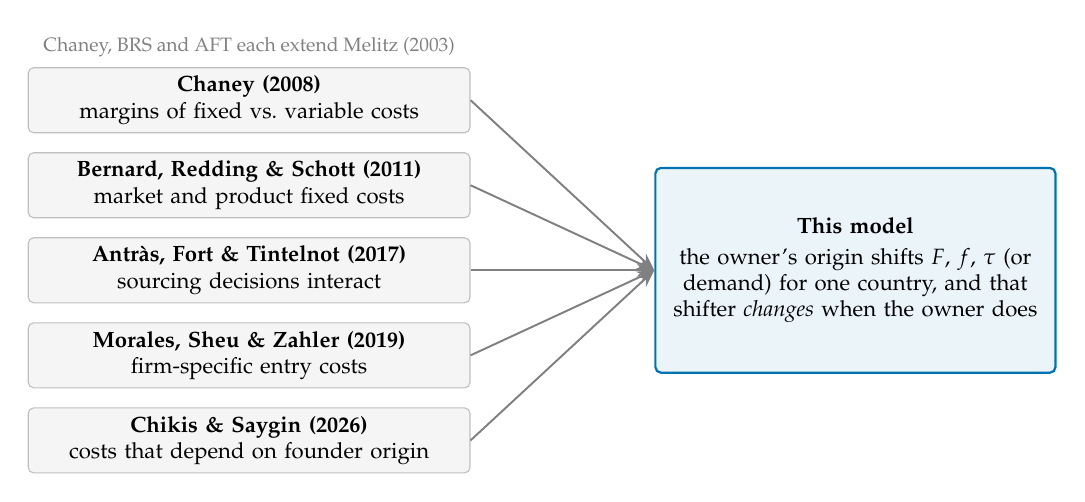
\begin{tikzpicture}[diag]
  \node[font=\scriptsize,color=gray] at (2.9,5.0) {Chaney, BRS and AFT each extend Melitz (2003)};
  \node[bx,text width=5.4cm,minimum height=0.8cm] (c) at (2.9,4.32) {\textbf{Chaney (2008)}\\ margins of fixed vs.\ variable costs};
  \node[bx,text width=5.4cm,minimum height=0.8cm] (b) at (2.9,3.24) {\textbf{Bernard, Redding \& Schott (2011)}\\ market and product fixed costs};
  \node[bx,text width=5.4cm,minimum height=0.8cm] (a) at (2.9,2.16) {\textbf{Antr\`as, Fort \& Tintelnot (2017)}\\ sourcing decisions interact};
  \node[bx,text width=5.4cm,minimum height=0.8cm] (m) at (2.9,1.08) {\textbf{Morales, Sheu \& Zahler (2019)}\\ firm-specific entry costs};
  \node[bx,text width=5.4cm,minimum height=0.8cm] (s) at (2.9,0.0) {\textbf{Chikis \& Saygin (2026)}\\ costs that depend on founder origin};
  \node[bxkey,text width=4.8cm,minimum height=2.6cm] (me) at (10.6,2.16)
     {\textbf{This model}\\[0.2em] the owner's origin shifts $F$, $f$, $\tau$ (or demand) for one country, and that shifter \emph{changes} when the owner does};
  \foreach \n in {c,b,a,m,s} \draw[arr] (\n.east) -- (me.west);
\end{tikzpicture}
\end{center}
\end{frame}


\begin{frame}{What is new is where the shifter enters, not the machinery}
\begin{enumerate}\setlength{\itemsep}{6pt}
\item<1-> \textbf{A person-specific, partner-specific friction}: costs differ by (owner origin, partner), not only by country pair or random draw
\item<2-> \textbf{It moves within a firm}: an ownership change switches it on, which gives a testable event
\item<3-> \textbf{Three channels in one setup}, with \emph{different} fingerprints, for imports \emph{and} exports, by product
\item<4-> \textbf{Two results for the design}: interdependence is absorbed within firm; diversification iff $s_{io}<H_i$
\end{enumerate}
\vspace{0.2cm}
\onslide<5->{\textcolor{gray}{Deliberately small: the aim is to tell channels apart with the data available, not to quantify welfare.}}
\end{frame}


\begin{frame}[label=compare]{No existing model pairs an owner-specific friction with a change in owner}
\scriptsize
\renewcommand{\arraystretch}{1.25}
\begin{tabularx}{\textwidth}{@{}>{\raggedright\arraybackslash}p{2.2cm}>{\raggedright\arraybackslash}p{3.0cm}YYp{1.3cm}>{\raggedright\arraybackslash}p{1.8cm}@{}}
\toprule
 & \textbf{Firm-specific bilateral cost?} & \textbf{Where it comes from} & \textbf{Moves within the firm?} & \textbf{Direction} & \textbf{Many partners?}\\
\midrule
Chaney (2008) & no: $\tau_{ij},f_{ij}$ by country pair & n/a (productivity) & n/a & exports & yes\\
BRS (2011) & no: $F_{ij},f_{ij}$ by country pair & n/a (ability) & n/a & exports & yes, + products\\
AFT (2017) & in estimation only & random draws & no & imports & yes\\
MSZ (2019) & yes: sunk entry cost & its own past exports & yes, by own choices & exports & yes\\
CS (2026) & yes: search cost $\kappa_{on}$ & founder's birthplace & no (the founder) & imports & 1 country per input\\
\midrule
\textbf{This model} & \textbf{yes}: $F,f,\tau$ & \textbf{owner's origin} & \textbf{yes: new owner} & \textbf{both} & \textbf{yes, + products}\\
\bottomrule
\end{tabularx}
\vspace{0.3cm}

\normalsize
Details:
\hyperlink{app-chaney}{\beamergotobutton{Chaney}}
\hyperlink{app-brs}{\beamergotobutton{BRS}}
\hyperlink{app-aft}{\beamergotobutton{AFT}}
\hyperlink{app-msz}{\beamergotobutton{MSZ}}
\hyperlink{app-cs}{\beamergotobutton{CS}}
\end{frame}


\begin{frame}{Why the existing models could not answer this question as built}
\small
\begin{itemize}\setlength{\itemsep}{5pt}
\item \textbf{Chaney; BRS}: trade costs are the same for every firm in a country pair. Firm heterogeneity (productivity, ability) raises trade with \emph{all} partners, so it has no country of origin
\item \textbf{AFT}: firm-by-country fixed costs appear only as random draws in estimation; nothing ties them to a person
\item \textbf{MSZ}: closest in spirit, with firm-specific entry costs. But the knowledge comes from the firm's own past exports, which it chooses itself
\item \textbf{CS}: costs tied to a person's origin, but the founder never changes and each input comes from one country, so there is no event and no partner count
\end{itemize}
\pause
\textcolor{gray}{Each could be extended to include an owner. The contribution is choosing where the shifter enters and deriving fingerprints that an ownership change can test.}
\end{frame}


\begin{frame}{Validation: the model reproduces its parents' results as special cases}
\footnotesize
\renewcommand{\arraystretch}{1.25}
\begin{tabularx}{\textwidth}{@{}>{\raggedright\arraybackslash}p{2.4cm}Y>{\raggedright\arraybackslash}p{4.2cm}@{}}
\toprule
\textbf{Source result} & \textbf{What it says} & \textbf{Our counterpart}\\
\midrule
Chaney (2008) & fixed costs have zero intensive-margin elasticity; variable costs move both margins & fixed-cost channel leaves existing flows unchanged\\
BRS (2011) & fixed costs affect whether to supply a market, not sales once supplied & product and country cutoffs\\
AFT (2017) & at $(\sigma-1)/\theta=1$, adding one source does not affect adding others & our separable baseline\\
\bottomrule
\end{tabularx}
\pause
\vspace{0.2cm}

\small
\textbf{Priors for $\lambda$}: shared language with a past destination cuts entry costs 29--36\% (MSZ); common language cuts fixed sourcing costs $\approx$13\% (AFT); birth-country search costs 33--78\% lower (CS).
\end{frame}


\begin{frame}{Where the model is weaker than its parents}
\begin{itemize}\setlength{\itemsep}{8pt}
\item \textbf{Static}: MSZ show that sunk costs and path dependence matter; here dynamics enter only through timing predictions
\item \textbf{No prices}: CS see founders reach cheaper suppliers; with trade values only, search and variable-cost cuts look alike
\item \textbf{Partial equilibrium}: no welfare or aggregate counterfactuals, unlike Chaney, AFT or CS
\end{itemize}
\pause
\vspace{0.2cm}
MSZ's ``extended gravity'' suggests an extension: the owner's knowledge may also lower costs in countries \emph{similar} to $o$ (language, region).
\end{frame}

%=====================================================================
\begin{transitionframe}
\centering\vfill{\Huge\bfseries Empirical Strategy}\vfill
\end{transitionframe}
%=====================================================================

\begin{frame}{Compare trade with $o$ to other countries, within firm and year}
\[
X_{ickt}=\exp\big(\textcolor{red}{\beta}\,\Post_{it}\times\mathbbm{1}[c=o_i]+\alpha_{it}+\gamma_{ckt}+\delta_{ick}\big)\,\epsilon_{ickt}
\]
\vspace{-0.3cm}
\begin{center}\small estimated by PPML, zeros kept, separately for imports and exports\end{center}
\footnotesize
\renewcommand{\arraystretch}{1.25}
\begin{tabularx}{\textwidth}{@{}p{4.6cm}Y@{}}
\toprule
\textbf{Fixed effect} & \textbf{Absorbs}\\
\midrule
firm $\times$ year $\alpha_{it}$ & everything a sale changes for the whole firm: management, finance, scale\\
country $\times$ product $\times$ year $\gamma_{ckt}$ & tariffs, trade agreements, exchange rates, demand in $c$\\
firm $\times$ country $\times$ product $\delta_{ick}$ & persistent fit with $c$, including buyers' selection on levels\\
\bottomrule
\end{tabularx}
\vspace{0.2cm}

\small
\textbf{Identifying assumption}: absent the switch, trade with $o$ relative to other countries would have evolved as in comparison firms.
\end{frame}


\begin{frame}{The event study and margin outcomes map onto the fingerprints}
\begin{columns}[T]
\begin{column}{0.47\textwidth}
\textbf{Event study}\\
{\small Stacked by cohort and origin with clean controls, event time $-4$ to $+6$; robust to staggered timing.}

\textbf{Inference}\\
{\small Firm clusters plus randomization inference with placebo origins.}
\end{column}
\begin{column}{0.47\textwidth}
\textbf{Margins}
\begin{itemize}\setlength{\itemsep}{2pt}\small
\item country entry: trades with $o$ at all?
\item product breadth with $o$
\item new $(o,k)$ pairs
\item existing $(o,k)$ flows {\scriptsize(zeros kept; no survivor conditioning)}
\end{itemize}
\textbf{Across firms}: {\small number of partners, HHI, non-U.S.\ share, third countries.}
\end{column}
\end{columns}
\vspace{0.2cm}
\hyperlink{fingerprints}{\beamergotobutton{Back to fingerprints}}
\end{frame}


\begin{frame}{A skeptic: buyers pick firms about to trade with $o$ anyway}
\footnotesize
\renewcommand{\arraystretch}{1.3}
\begin{tabularx}{\textwidth}{@{}>{\raggedright\arraybackslash}p{4.6cm}Y@{}}
\toprule
\textbf{Objection} & \textbf{Response}\\
\midrule
Buyer foresees growth with $o$ & event-study leads; drop switches with a pre-sale jump; compare with buyers from \emph{other} origins\\
Firms trading with $o$ attract buyers from $o$ & firm $\times$ country $\times$ product effects; results by pre-sale trading status\\
A sale reshuffles everything & firm $\times$ year effects; sales to non-immigrants as placebo\\
Early immigrants coded as non-immigrant & restrict by seller age; alternative ownership definitions \hyperlink{app-degree}{\beamergotobutton{Degree}}\\
Fake origins would ``work'' too & placebo origins far from $o$ in language and region\\
\bottomrule
\end{tabularx}
\note[item]{Residual risk: selection on firm-and-o-specific shocks that do not show up in the leads.}
\end{frame}

%=====================================================================
\begin{transitionframe}
\centering\vfill{\Huge\bfseries Results}\vfill
\end{transitionframe}
%=====================================================================

\begin{frame}{Trade with the owner's origin rises after the switch}
\begin{center}
\fbox{\parbox[c][3.6cm][c]{0.8\textwidth}{\centering\placeholder{Event-study figure, imports and exports side by side: $\beta_e$ for $e\in[-4,6]$ with 95\% CIs and the number of treated firms at each horizon.}}}
\end{center}
\textbf{How to read it}: flat leads support the design. A gradual rise points to fixed costs (search); a jump points to variable costs or demand.
\end{frame}


\begin{frame}{The increase comes mainly through the \_\_\_ margin}
\begin{center}
\fbox{\parbox[c][3.6cm][c]{0.8\textwidth}{\centering\placeholder{Effect on country entry, product breadth, new pairs and existing flows, by direction.}}}
\end{center}
\textbf{How to read it}: new pairs with flat existing flows point to fixed costs; proportional growth of existing flows points to variable costs.
\end{frame}


\begin{frame}{Firms' trade becomes \_\_\_ concentrated}
\begin{center}
\fbox{\parbox[c][3.6cm][c]{0.8\textwidth}{\centering\placeholder{Effects on number of partners, HHI, non-U.S.\ share, and trade with third countries (created vs.\ diverted).}}}
\end{center}
\textbf{How to read it}: rising third-country trade means sources are complements (AFT); falling means diversion.
\end{frame}


\begin{frame}{Conclusion}
\begin{beamercolorbox}[wd=\textwidth,sep=10pt,center,rounded=true,shadow=true]{questionbox}
\textbf{If owners carry market knowledge, who owns Canada's firms shapes where Canada trades.}
\end{beamercolorbox}
\vspace{0.3cm}
\begin{itemize}\setlength{\itemsep}{6pt}
\item \placeholder{An owner from $o$ is worth \_\_\% more trade with $o$}
\item \placeholder{Mostly through \_\_\_: evidence for the \_\_\_ channel}
\item \placeholder{The firm's concentration on the United States \_\_\_}
\end{itemize}
\end{frame}


\begin{frame}
\centering
\vspace{1cm}

{\Huge \textbf{Thank You}}
\vspace{0.5cm}

{\Large \textcolor{gray}{Questions \& Discussion}}
\vfill

\end{frame}

%=====================================================================
% BACKUP SLIDES
%=====================================================================
\appendix

\begin{frame}[label=app-chaney]{Chaney (2008): heterogeneous firms, fixed and variable export costs}
\begin{columns}[T]
\begin{column}{0.46\textwidth}
\small
Firms draw productivity $\varphi$ from a Pareto with shape $\gamma>\sigma-1$. Exporting from $i$ to $j$ costs iceberg $\tau_{ij}$ and fixed $f_{ij}$, the same for all firms in the pair. Only firms above a threshold export; firm exports have elasticity $\sigma-1$ with respect to $\tau_{ij}$.
\end{column}
\begin{column}{0.5\textwidth}
\footnotesize
Margins of aggregate exports (Section III):
\[
\zeta\equiv-\tfrac{d\ln X_{ij}}{d\ln\tau_{ij}}=\underbrace{\sigma-1}_{\text{int.}}+\underbrace{\gamma-(\sigma-1)}_{\text{ext.}}=\gamma
\]
\[
\xi\equiv-\tfrac{d\ln X_{ij}}{d\ln f_{ij}}=\underbrace{0}_{\text{int.}}+\underbrace{\tfrac{\gamma}{\sigma-1}-1}_{\text{ext.}}
\]
\end{column}
\end{columns}
\small
\textbf{Used here}: fixed costs move only the extensive margin. \textbf{Not here}: costs vary by country pair, not by owner.
\src{Chaney (2008), AER 98(4): eqs.\ 2--3, Propositions 1--2. \hyperlink{compare}{\beamerreturnbutton{Back}}}
\end{frame}


\begin{frame}[label=app-brs]{Bernard, Redding \& Schott (2011): fixed costs per market and per product}
\begin{columns}[T]
\begin{column}{0.46\textwidth}
\small
Firm ability $\varphi$ is common across products and countries; product attributes $\lambda$ are idiosyncratic. Serving market $j$ costs $F_{ij}$; each product there costs $f_{ij}$; trade costs are iceberg $\tau_{ij}$. A product is supplied if $\lambda\ge\lambda^*_{ij}(\varphi)$; a market is served if the profitable products cover $F_{ij}$.
\end{column}
\begin{column}{0.5\textwidth}
\footnotesize
Profits in market $j$ (eq.\ 9):
\begin{align*}
\pi_{ij}(\varphi)=&\int_{\lambda^*_{ij}(\varphi)}^{\infty}\Big(\tfrac{r_{ij}(\varphi,\lambda)}{\sigma}-w_if_{ij}\Big)z(\lambda)\,d\lambda\\
&-\,w_iF_{ij}
\end{align*}
\end{column}
\end{columns}
\small
\textbf{Used here}: the two-tier fixed-cost structure. \textbf{Not here}: $F_{ij},f_{ij}$ are common to all firms from $i$ to $j$.
\src{Bernard, Redding \& Schott (2011), QJE 126(3): Sections III.B--III.D, eqs.\ 6--10. \hyperlink{compare}{\beamerreturnbutton{Back}}}
\end{frame}


\begin{frame}[label=app-aft]{Antr\`as, Fort \& Tintelnot (2017): interdependent sourcing decisions}
\begin{columns}[T]
\begin{column}{0.5\textwidth}
\small
A firm pays $f_{ij}$ to source from $j$. Sourcing capability $\Theta_i=\sum_{j\in\mathcal J_i}T_j(\tau_{ij}w_j)^{-\theta}$; $j$'s share of input purchases is $T_j(\tau_{ij}w_j)^{-\theta}/\Theta_i$ (eqs.\ 7--8). If $(\sigma-1)/\theta\ge1$, sources are complements: a lower $\tau_{ij}$ or $f_{ij}$ weakly raises purchases from \emph{all} countries (Prop.\ 3). In estimation, fixed costs are lognormal draws by firm and country.
\end{column}
\begin{column}{0.46\textwidth}
\footnotesize
Profits (eq.\ 10):
\begin{align*}
\pi_i(\varphi)=&\,\varphi^{\sigma-1}(\gamma\Theta_i)^{\frac{\sigma-1}{\theta}}B_i\\
&-w_i\textstyle\sum_{j\in\mathcal J_i}f_{ij}
\end{align*}
\end{column}
\end{columns}
\small
\textbf{Used here}: third-country effects are common across partners. \textbf{Not here}: an owner; exports.
\src{Antr\`as, Fort \& Tintelnot (2017), AER 107(9); numbering from the resubmitted draft. \hyperlink{compare}{\beamerreturnbutton{Back}}}
\end{frame}


\begin{frame}[label=app-msz]{Morales, Sheu \& Zahler (2019): entry costs fall after similar markets}
\begin{columns}[T]
\begin{column}{0.5\textwidth}
\small
Chilean chemical exporters, 1995--2005; dynamic choice of destinations. Sunk entry costs fall if the destination shares a border, continent, language or income level with a country the firm exported to \emph{last year}. Moment inequalities: the model is not solved and there are no counterfactuals.
\end{column}
\begin{column}{0.46\textwidth}
\footnotesize
Sunk entry cost (eqs.\ 11--13):
\[
s_{ijt}=s_j^o-e^o_{ijt}+\varepsilon^S_{ijt}
\]
$e^o_{ijt}$: extended-gravity reductions. Jointly $-69$ to $-90\%$; geography $-25$ to $-38\%$; language $-29$ to $-36\%$.
\end{column}
\end{columns}
\small
\textbf{Used here}: firm-specific knowledge lowers market-specific entry costs. \textbf{Not here}: knowledge from a person; imports.
\src{Morales, Sheu \& Zahler (2019), REStud 86(6): Section 3. \hyperlink{compare}{\beamerreturnbutton{Back}}}
\end{frame}


\begin{frame}[label=app-cs]{Chikis \& Saygin (2026): founder origin lowers supplier search costs}
\begin{columns}[T]
\begin{column}{0.5\textwidth}
\small
Agents choose wage work or entrepreneurship. An entrepreneur buys one input from one country $n$ and searches sequentially for suppliers; each draw costs $P\kappa_{on}$ (founder origin $o$, source $n$). Sourcing odds identify relative search costs (Prop.\ 2), given equal domestic search costs. Birth-country search costs: 33--78\% below natives'.
\end{column}
\begin{column}{0.46\textwidth}
\footnotesize
Sourcing odds (eq.\ 15):
\[
\tfrac{\kappa_{on}/\kappa_{on'}}{\kappa_{o'n}/\kappa_{o'n'}}=\Big(\tfrac{\omega_{on}/\omega_{on'}}{\omega_{o'n}/\omega_{o'n'}}\Big)^{-\theta/\eta}
\]
Multi-input extension: one source per input (App.\ B.6).
\end{column}
\end{columns}
\small
\textbf{Used here}: person-origin-specific frictions. \textbf{Not here}: change of owner, exports, number of partners.
\src{Chikis \& Saygin (2026), job market paper: Sections 3.2--3.3, 4. \hyperlink{compare}{\beamerreturnbutton{Back}}}
\end{frame}


% Revived from the class deck: treatment intensity, plus the co-national hiring outcome
\begin{frame}[label=app-degree]{Effects by degree of immigrant ownership}
\begin{table}[h]
\centering
\renewcommand{\arraystretch}{1.3}
\footnotesize
\begin{tabular}{lccc}
\toprule
 & \textbf{At Least One} & \textbf{Majority} & \textbf{Full} \\
 & \textbf{Immigrant Owner} & \textbf{Immigrant} & \textbf{Immigrant} \\
\midrule
Trade with $o$: $\Post\times\mathbbm{1}[c=o]$ & & & \\
 & \textit{(s.e.)} & \textit{(s.e.)} & \textit{(s.e.)} \\
Fraction of immigrant workers & & & \\
 & \textit{(s.e.)} & \textit{(s.e.)} & \textit{(s.e.)} \\
\midrule
Observations & & & \\
\bottomrule
\multicolumn{4}{l}{\scriptsize \textit{Notes:} Row 2 tests co-national hiring. SEs clustered by firm.} \\
\end{tabular}
\end{table}
\hyperlink{preview}{\beamergotobutton{Back to Preview}}
\end{frame}


\begin{frame}{Proofs in one line each}
\small
\begin{itemize}\setlength{\itemsep}{6pt}
\item \textbf{Margins.} Fixed-cost cuts leave $\Phi\tau^{-\varepsilon}$ unchanged, so existing flows are unchanged; only the cutoffs move. A variable-cost cut raises every $X_{iok}$ by $\varepsilon\lambda_\tau\iota_o$ in logs.
\item \textbf{Country fixed cost.} If $\Omega_{iod}\ge F_{iod}$ already held, nothing changes; otherwise entry activates every $k$ with $\Phi\tau^{-\varepsilon}\ge f$ at once.
\item \textbf{Diversification.} $H=\sum X_c^2/X^2\Rightarrow\partial H/\partial X_o=2(s_o-H)/X$.
\item \textbf{Interdependence.} $M_{ij}\propto T_j(\tau_{ij}w_j)^{-\theta}\Theta_i^{(\sigma-1-\theta)/\theta}$: a cut in $\tau_{io}$ scales all $j\neq o$ equally; $\ln M_{io}-\ln M_{ij}$ rises by $\theta\lambda_\tau\iota_o$.
\end{itemize}
\end{frame}

\end{document}
